\documentclass[11pt,a4paper]{article}
\usepackage[a4paper,margin=2.5cm,headheight=14pt,footskip=1.2cm]{geometry}
\usepackage{graphicx}
\usepackage{xcolor}
\usepackage{amsmath}
\usepackage{booktabs,tabularx,array}
\usepackage{etoolbox}
\usepackage{tikz}
\usetikzlibrary{positioning,arrows.meta,shapes.geometric,calc,fit,backgrounds}
\usepackage{titlesec}
\usepackage{fancyhdr}
\usepackage{enumitem}
\usepackage[labelfont={bf,color=iris},font=small,skip=5pt]{caption}
\usepackage[round,authoryear]{natbib}
\usepackage[colorlinks,linkcolor=iris,citecolor=iris,urlcolor=iris]{hyperref}

% the chart files in slides/charts load their images as img/..., so slides/ comes first
\graphicspath{{../slides/}{../docs/img/}{../slides/img/}}

% same palette as slides/main.tex: ink is the indigo of the IIT Kharagpur logo
\definecolor{bg}{HTML}{F6F5FB}
\definecolor{ink}{HTML}{291973}
\definecolor{iris}{HTML}{5B4FB0}
\definecolor{saffron}{HTML}{B45309}
\definecolor{gold}{HTML}{F2C14E}
\definecolor{haze}{HTML}{EEECF7}
\definecolor{muted}{HTML}{6C6889}
\definecolor{rule}{HTML}{D5D1E8}
\definecolor{cbuilt}{HTML}{D7302A}
\definecolor{cveg}{HTML}{1A9850}
\definecolor{copen}{HTML}{E2CF7A}
\definecolor{cwater}{HTML}{3B7DB8}

\tikzset{
  every picture/.append style={text=ink},
  card/.style={rounded corners=3pt,fill=haze,draw=rule,line width=.4pt,align=left},
  step/.style={rounded corners=3pt,fill=white,draw=rule,line width=.5pt,align=left,
    text width=#1,inner sep=4pt,font=\scriptsize},
  step/.default=2.55cm,
  flowarrow/.style={-{Stealth[length=2.2mm]},line width=.9pt,iris},
  num/.style={circle,fill=saffron,text=white,font=\scriptsize\bfseries,inner sep=1.5pt,minimum size=4.5mm},
}
\newcommand{\capt}[1]{{\color{iris}\scriptsize\bfseries #1}}
\newcommand{\sw}[1]{\tikz[baseline=-.6ex]\fill[#1] (0,0) circle (2.2pt);}
\newcommand{\classlegend}{\sw{cbuilt}\,Built-up\quad\sw{cveg}\,Vegetation\quad\sw{copen}\,Open land\quad\sw{cwater}\,Water}
\makeatletter
\newcommand{\ra}{\ifdefequal{\f@series}{\bfdefault}{{\boldmath$\rightarrow$}}{$\rightarrow$}}
\makeatother
\newcommand{\keybox}[2][haze]{\par\noindent\begin{tikzpicture}\node[card,fill=#1,text width=\dimexpr\linewidth-12.4pt\relax,inner sep=6pt,font=\small]{#2};\end{tikzpicture}\par}
\titleformat{\section}{\color{ink}\Large\bfseries}{\color{saffron}\thesection}{.75em}{}
\titleformat{\subsection}{\color{ink}\large\bfseries}{\color{saffron}\thesubsection}{.7em}{}
\titlespacing*{\section}{0pt}{3ex plus 1ex minus .2ex}{1.4ex plus .2ex}

\pagestyle{fancy}
\fancyhf{}
\renewcommand{\headrulewidth}{0pt}
\renewcommand{\footrulewidth}{.6pt}
\renewcommand{\footrule}{{\color{gold}\vskip-\footruleskip\vskip-\footrulewidth\hrule width\headwidth height\footrulewidth\vskip\footruleskip}}
\fancyfoot[L]{\color{muted}\scriptsize Indian Institute of Technology Kharagpur \quad CS60111 GIS Term Project, Group 8 \quad LULC change 2020-2025}
\fancyfoot[R]{\color{saffron}\small\bfseries\thepage}

\setlist[itemize]{label=\textcolor{saffron}{\rule[.25ex]{.9ex}{.9ex}},leftmargin=1.4em,itemsep=2pt,topsep=4pt}
\setlist[enumerate]{leftmargin=1.6em,itemsep=2pt,topsep=4pt}
\renewcommand{\arraystretch}{1.12}
\newcolumntype{Y}{>{\raggedright\arraybackslash}X}

\hypersetup{pdftitle={Land Use / Land Cover Mapping and Change Detection, IIT Kharagpur campus, 2020 vs 2025},pdfauthor={Ashutosh Sharma, Krishnkant Sahu, Sanskar Sovitkar}}
% floats, footnotes and TikZ text reset to \normalcolor, so ink has to be the default colour, not just the current one
\makeatletter
\AtBeginDocument{\color{ink}\let\default@color\current@color}
\makeatother

\begin{document}

% ---------------------------------------------------------------- title page, same layout ideas as the deck's first slide
\begin{titlepage}
\begin{tikzpicture}[remember picture,overlay]
  \fill[ink] (current page.north west) rectangle ([yshift=-9.4cm]current page.north east);
  \fill[gold] ([yshift=-9.4cm]current page.north west) rectangle ([yshift=-9.6cm]current page.north east);
  \node[anchor=north west,inner sep=0] (logo) at ([xshift=2.5cm,yshift=-1.5cm]current page.north west) {\includegraphics[height=1.9cm]{img/iitkgp_logo_white}};
  \node[anchor=west,text=white,font=\large\bfseries,align=left] at ([xshift=4mm]logo.east) {Indian Institute of\\Technology Kharagpur};
  \node[anchor=north west,text width=16cm,text=white,align=left,inner sep=0] at ([xshift=2.5cm,yshift=-4.4cm]current page.north west) {%
    {\color{gold}\small\bfseries CS60111 GIS \textperiodcentered\ TERM PROJECT REPORT \textperiodcentered\ GROUP 8\par}\vspace{3mm}
    {\fontsize{24}{29}\selectfont\bfseries Land Use / Land Cover Mapping\\and Change Detection\par}\vspace{3mm}
    {\large IIT Kharagpur campus, 2020 vs 2025, from multi-temporal Sentinel-2\par}};
  \node[anchor=south,text=muted,font=\small] at ([yshift=-11.0cm]current page.north) {2025 land cover map, Random Forest, 10~m};
  \node[anchor=north,inner sep=0] (tmap) at ([yshift=-11.2cm]current page.north) {\includegraphics[width=16cm]{img/lulc_2025.png}};
  \node[anchor=north] at ([yshift=-1mm]tmap.south) {\classlegend};
  \node[anchor=south west,inner sep=0,align=left] at ([xshift=2.5cm,yshift=2.6cm]current page.south west) {%
    \begin{tabular}{@{}l@{\hspace{6mm}}l@{}}
      \bfseries Ashutosh Sharma & 23CS10005\\
      \bfseries Krishnkant Sahu & 23CS10035\\
      \bfseries Sanskar Sovitkar & 24CS10131
    \end{tabular}};
  \node[anchor=south east,inner sep=0,align=right,font=\small] at ([xshift=-2.5cm,yshift=2.6cm]current page.south east) {%
    CS60111 Geographical Information System\\Autumn 2026-27, term project 3\\{\color{saffron}\bfseries November 2026}};
\end{tikzpicture}
\end{titlepage}

% ---------------------------------------------------------------- abstract
\section*{Abstract}
We mapped land use and land cover on the 469.2~ha fenced campus of IIT Kharagpur for the 2019-20 and 2024-25 dry seasons and measured what changed between them. Four classes (built-up, vegetation, open land, water) were mapped at 10~m from 51 cloud-screened Sentinel-2 scenes, using a winter and a pre-monsoon median composite for each year and 23 features per pixel. One Random Forest of 500 trees, trained on 556 points labelled by eye on WorldView-2 and WorldView-3 imagery, classified both years, so the same rules apply at both dates.

Accuracy was checked on 365 independent WorldView points drawn as a stratified random sample and is reported with area weights: 0.74 (95\% CI 0.64-0.84) for 2020 and 0.80 (0.71-0.89) for 2025. After a 30~m minimum-width filter, 51.0~ha (10.9\% of the campus) changed class. Most of it was open land: 30.8~ha became vegetation and 11.1~ha became built-up, 6.2~ha of that at one construction compound in the south-east, which a map per winter dates to clearing in 2020 and roofing by early 2023. Error-adjusted areas put the vegetation gain at $+94 \pm 66$ ha, the only net change larger than the map's own error. Across four tuning runs, the largest accuracy gain came from replacing Dynamic World training labels with our own. Radar, image embeddings and texture added nothing.

\vspace{3mm}
\keybox{%
  \begin{tabular}{@{}p{3.3cm}@{\hspace{4mm}}p{11.3cm}@{}}
  \textcolor{saffron}{\Large 51.0~ha} & changed (10.9\%): 30.8 open \ra{} vegetation, 11.1 open \ra{} built-up\\[2mm]
  \textcolor{saffron}{\Large $+$28.7 / $-$38.2} & net hectares of vegetation and open land; built-up $+$9.4~ha\\[2mm]
  \textcolor{saffron}{\Large 0.74 / 0.80} & overall accuracy 2020 / 2025 on 365 points, up from 0.67 / 0.77\\[2mm]
  \textcolor{saffron}{\Large 2020 \ra{} 2023} & the south-east compound: cleared in 2020, roofed by early 2023
  \end{tabular}}

\vspace{4mm}
{\setcounter{tocdepth}{1}\small\tableofcontents}

\clearpage
% ---------------------------------------------------------------- introduction
\section{Introduction and objectives}

\textbf{Research question.} How much of the 469~ha campus changed land cover between the 2019-20 and 2024-25 dry seasons, and from what to what?

Global 10~m land cover products such as Dynamic World \citep{brown2022} and ESA WorldCover are built for regions and continents. They are rarely checked at the scale where a campus estate office makes its decisions: one construction compound, one lawn, one pond. A campus of 469~ha is small enough to label by eye on very high resolution imagery and large enough to hold every class that matters, which makes it a fair test of whether a 10~m map can measure change there, and how well.

The project had four objectives:
\begin{enumerate}
  \item Map four campus classes at two dates from Sentinel-2 \citep{drusch2012} with one Random Forest \citep{breiman2001}.
  \item Produce a from-to change table in hectares, with a 30~m minimum change width so that pixel jitter is not reported as change.
  \item Assess accuracy against independent points labelled on WorldView-2 and WorldView-3 imagery, with area-weighted estimators and confidence intervals \citep{olofsson2014}.
  \item Keep the whole pipeline reproducible: one Google Earth Engine script \citep{gorelick2017} and one Python runner that rebuilds every number in this report.
\end{enumerate}

Since the mid-term evaluation we replaced the training labels (run 4), tested them against more input data, dated the largest construction site year by year, split the change into gain, loss and swap, and tested whether each class's net change is larger than the map error.

% ---------------------------------------------------------------- literature
\section{Literature review}
{\color{muted}\small This section is Sanskar Sovitkar's review (\path{literature/literature_README.md} in the repository), also slide 4 of the mid-term deck.}\medskip

Six studies on Sentinel-2 or Landsat land cover mapping and change detection were reviewed. Table~\ref{tab:lit} summarises five of them; the sixth, \citet{zhang2021}, classified urban land cover in Beijing from a single Sentinel-2 date with an optimised Random Forest (OA 98.3\%, kappa 0.975).

\begin{table}[htbp]
\centering\footnotesize
\caption{Studies reviewed (Sanskar Sovitkar). Reported accuracies are not directly comparable across studies: the class schemes, scales and validation methods differ.}
\label{tab:lit}
\begin{tabularx}{\linewidth}{@{}>{\raggedright\arraybackslash}p{2.6cm}Y>{\centering\arraybackslash}p{1.1cm}YY@{}}
\toprule
Paper & Data & Classes & Method & Accuracy\\
\midrule
\citet{tikuye2023} & Landsat, 1983, 2003, 2022; Upper Blue Nile Basin & 7 & Random Forest, change detection & Kappa 83 / 85 / 91\%\\
\citet{abdi2020} & Sentinel-2, multi-temporal; south-central Sweden & 8 & SVM, RF, XGBoost, deep learning compared & OA: SVM 75.8, XGBoost 75.1, RF 73.9, DL 73.3\%\\
\citet{alonso2021} & Sentinel-2, 12 monthly images of 2019; Galicia, Spain & 8 & One common Random Forest, 20~m & OA 91.6\%, kappa 0.90\\
\citet{rynkiewicz2023}, conference abstract & Sentinel-2 annual data, 2018-2021; Lodz (Poland) and Viken (Norway), on Google Earth Engine & 3 (change classes) & Spectral signatures, then Random Forest & OA $\geq$ 0.97, kappa $>$ 0.95\\
\citet{jagannathan2025} & Sentinel-2A/B, 2017-2024; Katpadi, Tamil Nadu & 8 & IRUNet deep learning with test-time augmentation & Pixel accuracy 98.21\%, F1 91.85\%, kappa 0.872\\
\bottomrule
\end{tabularx}
\end{table}

Three points from the review shaped the method. Random Forest is the common baseline and stays within about two points of SVM, XGBoost and deep learning on the same Sentinel-2 data \citep{abdi2020}, so a better classifier was not where the gains would be. \citet{alonso2021} trained one common forest across a multi-temporal stack, the same choice we made for 2020 and 2025 (Section~\ref{sec:method}). And every study works at basin, region or town scale with seven or eight classes. None maps a single campus, which is the gap this project tests: whether the 10~m approach holds on a few hundred hectares, where one compound or one lawn is a large share of the area.

% ---------------------------------------------------------------- study area
\section{Study area}

The study area is the main fenced campus of IIT Kharagpur, West Bengal (about 22.31\textdegree\,N, 87.31\textdegree\,E), taken from OpenStreetMap way 52435606, a 184-vertex polygon of 469.2~ha (Figure~\ref{fig:study}). Halls of residence and staff quarters outside the fence are not in it. One Sentinel-2 tile, 45QWE, covers the whole campus, and all outputs are exported in UTM zone 45N (EPSG:32645) at 10~m.

\begin{figure}[htbp]
\centering
\includegraphics[width=.86\linewidth]{img/study_area-04.png}
\caption{Study area: the OSM campus boundary on Google Earth imagery (Airbus), with north arrow and scale bar. Figure by Sanskar Sovitkar.}
\label{fig:study}
\end{figure}

% ---------------------------------------------------------------- data
\section{Data}

Table~\ref{tab:data} lists the inputs. Both years use the same two seasons, so seasonal greening is not counted as change. The pre-monsoon composite exists because by April the lawns have dried out while tree canopy stays green, which separates two classes that look alike in winter.

\begin{table}[htbp]
\centering\small
\caption{Data used.}
\label{tab:data}
\begin{tabularx}{\linewidth}{@{}>{\raggedright\arraybackslash}p{3.2cm}Y@{}}
\toprule
Item & Value\\
\midrule
Imagery & Sentinel-2 L2A, \path{COPERNICUS/S2_SR_HARMONIZED}, 10 bands (B2-B8A, B11, B12), tile 45QWE\\
Epoch 1 & 1 Nov 2019 to 29 Feb 2020 (winter), 11 scenes; 1 Mar to 31 May 2020 (pre-monsoon), 11 scenes\\
Epoch 2 & 1 Nov 2024 to 28 Feb 2025, 16 scenes; 1 Mar to 31 May 2025, 13 scenes\\
Scene filter & tile cloud $<$ 40\%, then cloud inside the campus $<$ 10\% (winter) or $<$ 20\% (pre-monsoon, hazier), from the SCL band\\
Training labels & 556 points labelled by eye on WorldView-2 (15 Mar 2020) and WorldView-3 (13 Jan 2024)\\
Validation labels & 365 independent points on the same WorldView scenes (Esri World Imagery Wayback), labelled by Krishnkant Sahu\\
Comparison map & Dynamic World V1, \path{GOOGLE/DYNAMICWORLD/V1}, modal label over the same windows; runs 1-3 trained on it\\
Boundary & OpenStreetMap way 52435606, \path{data/iitkgp_campus_osm.geojson}\\
Export grid & UTM 45N, EPSG:32645, 10~m\\
\bottomrule
\end{tabularx}
\end{table}

\begin{figure}[htbp]
\centering
\begin{minipage}[t]{.49\linewidth}\centering
  \includegraphics[width=\linewidth]{img/true_colour_2020.png}\\\capt{Winter 2019-20 median composite, 11 scenes}
\end{minipage}\hfill
\begin{minipage}[t]{.49\linewidth}\centering
  \includegraphics[width=\linewidth]{img/true_colour_2025.png}\\\capt{Winter 2024-25 median composite, 16 scenes}
\end{minipage}\\[4mm]
\begin{tikzpicture}\input{../slides/charts/timeline}\end{tikzpicture}
\caption{Top: true-colour winter composites. Bottom: every scene that passed the campus cloud test, by season. 51 scenes in all.}
\label{fig:data}
\end{figure}

% ---------------------------------------------------------------- classes
\section{Classes}

Four classes cover the campus (Table~\ref{tab:classes}, Figure~\ref{fig:chips}). They are coarser than the eight or nine classes of global products on purpose: each one is a class the 10~m pixel can actually separate, and each matters for planning.

\begin{table}[htbp]
\centering\small
\caption{Class scheme and the Dynamic World labels mapped to each class for comparison.}
\label{tab:classes}
\begin{tabularx}{\linewidth}{@{}cl Y >{\raggedright\arraybackslash}p{4.2cm}@{}}
\toprule
Code & Class & What goes in it & Dynamic World labels\\
\midrule
0 & \sw{cbuilt}\,Built-up & Roofs, roads, paved courts, parking & built\\
1 & \sw{cveg}\,Vegetation & Tree canopy, dense scrub, flooded vegetation & trees, flooded vegetation\\
2 & \sw{copen}\,Open land & Lawns, playgrounds, dry grassland, bare soil, cleared plots & grass, crops, shrub and scrub, bare\\
3 & \sw{cwater}\,Water & Ponds, tanks, open drains wide enough to fill a 10~m pixel & water\\
\bottomrule
\end{tabularx}
\end{table}

\begin{figure}[htbp]
\centering
\begin{tikzpicture}
  \foreach \i/\n/\c/\d in {0/Built-up/cbuilt/roofs{,} roads{,} courts,1/Vegetation/cveg/canopy{,} dense woody,2/Open land/copen/lawns{,} fields{,} bare plots,3/Water/cwater/ponds{,} tanks}{
    \node[anchor=north west,inner sep=0] (im\i) at (4.05*\i,0) {\includegraphics[width=3.75cm]{img/chip\i-07.png}};
    \fill[\c] (im\i.south west) rectangle ([yshift=-1.2mm]im\i.south east);
    \node[anchor=north west,font=\small\bfseries,inner sep=1pt] at ([yshift=-1.8mm]im\i.south west) {\n};
    \node[anchor=north west,font=\scriptsize,text=muted,inner sep=1pt] at ([yshift=-6mm]im\i.south west) {\d};
  }
\end{tikzpicture}
\caption{Example of each class on WorldView imagery.}
\label{fig:chips}
\end{figure}

\textbf{The crops rule.} Dynamic World almost never says ``grass'' on this campus (0.6~ha in 2020). It labels the lawns and sports fields as crops, about 50~ha in 2020. There is no farmland inside the fence, so crops go to open land; putting them in vegetation would hide exactly the open-to-built conversions this project looks for. Dynamic World's ``shrub and scrub'' on campus is the dry grassland with scattered bushes in the east end, which the independent points label open land, so it goes to open land too. Runs 1-3 trained on this remap. The final map trains on points labelled directly in the four classes and uses the remap only to compare with Dynamic World.

% ---------------------------------------------------------------- method
\section{Method}
\label{sec:method}

Figure~\ref{fig:pipeline} shows the pipeline end to end. It runs in Google Earth Engine as one script (\path{gee/lulc_pipeline.js}), and the same steps run through the Python API in \path{scripts/run_pipeline.py}, which writes \path{results/results.json}. Every number in this report comes from that file or from the two analysis outputs named in Section~\ref{sec:code}.

\begin{figure}[htbp]
\centering
\resizebox{\linewidth}{!}{%
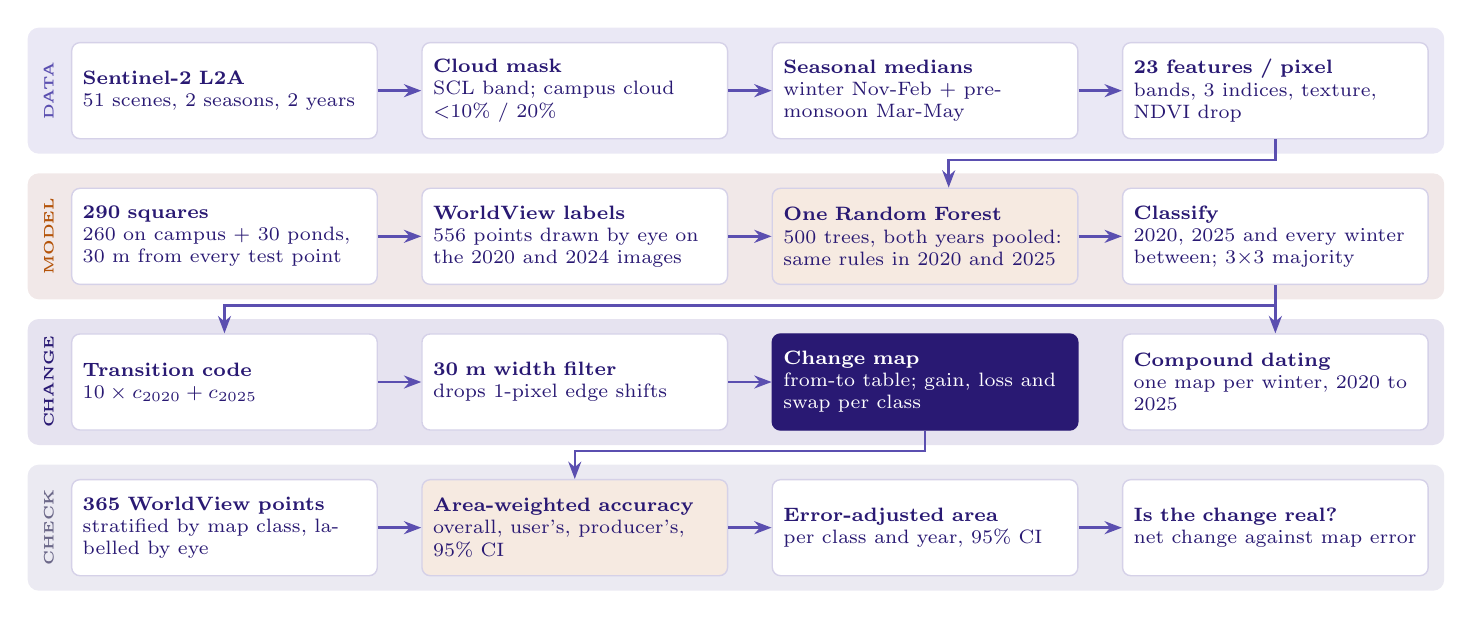
\begin{tikzpicture}[node distance=5.5mm,step/.append style={text width=3.6cm,minimum height=1.22cm}]
  \foreach \y/\c/\t in {0/iris/DATA,-1.85/saffron/MODEL,-3.7/ink/CHANGE,-5.55/muted/CHECK}{
    \fill[\c!8!bg,rounded corners=4pt] (0,\y+.8) rectangle (17.99,\y-.8);
    \node[rotate=90,font=\tiny\bfseries,text=\c] at (.27,\y) {\t};
  }
  \node[step,anchor=west] (s1) at (.55,0) {\textbf{Sentinel-2 L2A}\\51 scenes, 2 seasons, 2 years};
  \node[step,right=of s1] (s2) {\textbf{Cloud mask}\\SCL band; campus cloud $<$10\% / 20\%};
  \node[step,right=of s2] (s3) {\textbf{Seasonal medians}\\winter Nov-Feb + pre-monsoon Mar-May};
  \node[step,right=of s3] (s4) {\textbf{23 features / pixel}\\bands, 3 indices, texture, NDVI drop};
  \node[step,anchor=west] (m1) at (.55,-1.85) {\textbf{290 squares}\\260 on campus + 30 ponds, 30~m from every test point};
  \node[step,right=of m1] (m2) {\textbf{WorldView labels}\\556 points drawn by eye on the 2020 and 2024 images};
  \node[step,right=of m2,fill=saffron!12] (m3) {\textbf{One Random Forest}\\500 trees, both years pooled: same rules in 2020 and 2025};
  \node[step,right=of m3] (m4) {\textbf{Classify}\\2020, 2025 and every winter between; 3$\times$3 majority};
  \node[step,anchor=west] (c1) at (.55,-3.7) {\textbf{Transition code}\\$10\times c_{2020} + c_{2025}$};
  \node[step,right=of c1] (c2) {\textbf{30~m width filter}\\drops 1-pixel edge shifts};
  \node[step,right=of c2,fill=ink,text=white,draw=ink] (c3) {\textbf{Change map}\\from-to table; gain, loss and swap per class};
  \node[step,right=of c3] (c4) {\textbf{Compound dating}\\one map per winter, 2020 to 2025};
  \node[step,anchor=west] (k1) at (.55,-5.55) {\textbf{365 WorldView points}\\stratified by map class, labelled by eye};
  \node[step,right=of k1,fill=saffron!12] (k2) {\textbf{Area-weighted accuracy}\\overall, user's, producer's, 95\% CI};
  \node[step,right=of k2] (k3) {\textbf{Error-adjusted area}\\per class and year, 95\% CI};
  \node[step,right=of k3] (k4) {\textbf{Is the change real?}\\net change against map error};
  \foreach \a/\b in {s1/s2,s2/s3,s3/s4,m1/m2,m2/m3,m3/m4,c1/c2,c2/c3,k1/k2,k2/k3,k3/k4}{\draw[flowarrow] (\a) -- (\b);}
  \draw[flowarrow] (s4.south) -- ++(0,-.26) -| ($(m3.north)+(.3,0)$);
  \draw[flowarrow] (m4.south) -- ++(0,-.26) -| (c1.north);
  \draw[flowarrow] (m4) -- (c4);
  \draw[flowarrow] (c3.south) -- ++(0,-.26) -| (k2.north);
\end{tikzpicture}}
\caption{From 51 Sentinel-2 scenes to a tested from-to change table.}
\label{fig:pipeline}
\end{figure}

\subsection{Composites and features}
Each scene is masked with its scene classification layer (SCL classes 1, 3, 8, 9 and 10: saturated, cloud shadow, medium and high cloud, cirrus), and the median is taken per season. Each pixel then gets 23 features:
\begin{itemize}
  \item the 10 winter bands (B2-B8A, B11, B12) and three winter indices,
  \[
  \mathrm{NDVI}=\frac{B8-B4}{B8+B4},\qquad
  \mathrm{NDBI}=\frac{B11-B8}{B11+B8},\qquad
  \mathrm{NDWI}=\frac{B3-B8}{B3+B8},
  \]
  for greenness, built-up surfaces and water, each separating a pair of classes that look alike in raw bands;
  \item texture: the 3$\times$3 standard deviation of NDVI and of B8, since canopy is rough and lawns are smooth;
  \item B4, B8, B11, B12 and the three indices from the pre-monsoon composite;
  \item the NDVI drop from winter to pre-monsoon: grass dries out by May, trees stay green.
\end{itemize}
The seasonal and texture features were added in run 3 to tell a lawn under scattered trees from canopy, and they rank high in the final forest (Figure~\ref{fig:importance}). The ranking is flat, all ten within 10\% of the top, so no single feature carries the map.

\begin{figure}[htbp]
\centering
\begin{tikzpicture}\input{../slides/charts/importance}\end{tikzpicture}\\[2mm]
{\small\sw{saffron} pre-monsoon \quad \sw{iris} texture \quad \sw{muted} winter}
\caption{Random Forest importance (Gini), top 10 of 23 features. The top two are 3$\times$3 texture of NDVI and NIR; 5 of the top 10 are seasonal or texture features.}
\label{fig:importance}
\end{figure}

\subsection{Training labels}
We drew 290 training locations: 260 at random inside the fence and 30 ponds within 3~km outside it, because the campus ponds are already covered by validation points. Each location was labelled by eye on the 2020 and the 2024 WorldView image wherever its 10~m square held one class, giving 286 points for 2020 and 270 for 2025 (87 built-up, 274 vegetation, 143 open land, 52 water). Every training point is at least 30~m from every validation point. Before labelling, 24 validation points were relabelled blind and 22 matched. The training stack reaches 3.5~km past the fence so the ponds have pixel values; the maps stay clipped to the campus.

\subsection{Classifier}
One Random Forest (500 trees, seed 42) is trained on the points of both epochs together and applied to both composites. Two separately trained forests disagree on the same unchanged pixel, and that disagreement shows up as fake change: a first run done that way reported 91~ha of built-up turning into vegetation. Both class maps then pass a 3$\times$3 majority filter. The out-of-bag error is 0.19 on the 556 training points.

\subsection{Change detection}
Change is post-classification. Each pixel gets the transition code $c = 10\,c_{2020} + c_{2025}$, so 21 is open land to vegetation and 11 is unchanged vegetation. A changed pixel counts only if it survives a one-pixel erosion of the change mask, after which the mask is dilated back. This drops changed strips narrower than about 30~m. Without it every roof gets a ring of change from the one-pixel boundary shift between the two composites: the raw change map holds 91.4~ha, the filtered one 51.0~ha.

For each class $k$ the from-to table gives gross gain $G_k$ and loss $L_k$, net change $G_k - L_k$, and swap $S_k = 2\min(G_k, L_k)$, the area that changed place without changing the class total \citep{pontius2004}.

\subsection{Accuracy assessment}
\label{sec:accmethod}
Krishnkant Sahu drew and labelled the independent validation set: 365 points, 181 for 2020 and 184 for 2025, a stratified random sample on the map classes with at least 33 points per class per year (40 / 40 / 40 / 61 and 33 / 40 / 39 / 72 for built-up / vegetation / open land / water). Each point was labelled on WorldView-2 (15 March 2020) or WorldView-3 (13 January 2024) imagery from Esri World Imagery Wayback, after correcting the imagery's offset to the Sentinel-2 grid (Figure~\ref{fig:valpoints}). None of these points was used for training.

Water is 0.2\% of the campus but a third of the points, so raw point counts would let water set the score. Every estimate is therefore weighted by stratum area \citep{olofsson2014}. With strata equal to map classes, stratum $i$ covering a share $W_i$ of the area $A$ and $n_{ij}$ points of map class $i$ and reference class $j$,
\[
\hat p_{ij} = W_i\,\frac{n_{ij}}{n_{i\cdot}},\qquad
\mathrm{OA}=\sum_j \hat p_{jj},\qquad
\mathrm{UA}_i=\frac{\hat p_{ii}}{\hat p_{i\cdot}},\qquad
\mathrm{PA}_j=\frac{\hat p_{jj}}{\hat p_{\cdot j}},\qquad
\hat A_j = A\,\hat p_{\cdot j},
\]
and the 95\% interval of $\hat A_j$ is $\pm 1.96\,A\,\sqrt{\sum_i W_i^2\, \frac{n_{ij}}{n_{i\cdot}}\big(1-\frac{n_{ij}}{n_{i\cdot}}\big)/(n_{i\cdot}-1)}$. The sample was drawn on the classes of an earlier map, and the final map no longer matches those strata, so we use the general form of \citet{stehman2014}: each point is weighted by the area of the stratum it was drawn from, not by its class on the current map.

Agreement with Dynamic World on 883 held-out pixels is also reported. It measures closeness to another map, not accuracy.

\textbf{Is the change real?} The 2020 and 2025 point sets are independent, so the error-adjusted net change of a class is $\hat A_{2025} - \hat A_{2020}$ and its 95\% half-width adds in quadrature, $h=\sqrt{h_{2020}^2+h_{2025}^2}$. A change is distinguishable from map error when the interval excludes zero.

\textbf{Tuning without overfitting the points.} Every change to the method after the first independent check was chosen on the odd-numbered validation points only, with the even-numbered half held out, by a rule fixed before the runs (best mean OA of both years on the odd half).

\begin{figure}[htbp]
\centering
\includegraphics[width=\linewidth]{img/08_validation_points.png}
\caption{The 365 independent validation points, 181 for 2020 and 184 for 2025, labelled by Krishnkant Sahu. Every training point is at least 30~m away from them.}
\label{fig:valpoints}
\end{figure}

% ---------------------------------------------------------------- tuning
\section{Model tuning}
\label{sec:tuning}

The final map is the fourth run. Each run fixed one measured error of the one before it (Table~\ref{tab:runs}).

\begin{table}[htbp]
\centering\small
\caption{Tuning runs. OA is area-weighted on the independent points, 2020 / 2025.}
\label{tab:runs}
\begin{tabularx}{\linewidth}{@{}l>{\raggedright\arraybackslash}p{4.6cm}Y>{\raggedleft\arraybackslash}p{1.5cm}@{}}
\toprule
Run & What changed & What it left, or fixed & Changed ha\\
\midrule
1 Baseline & Equal samples per class, one forest per year & Built-up 224~ha where Dynamic World says about 110; 91~ha built-up \ra{} vegetation on unchanged roofs; no open-land samples in 2020 & 139\\
2 Sampling & Samples near class shares (300 / 700 / 150 / 40); one forest for both years; crops \ra{} open land; 30~m change filter & Open land 32~ha, where the points say about 146; OA 0.61 / 0.74 & 48.6\\
3 Open land & Pre-monsoon composite, 3$\times$3 texture, shrub \ra{} open land, 450 open-land samples & Open land 103~ha; OA 0.67 / 0.77 & 71.4\\
\textbf{4 Labels (final)} & 556 points we labelled on WorldView replace Dynamic World as the label source; 500 trees & Open land 156~ha; \textbf{OA 0.74 / 0.80} & \textbf{51.0}\\
\bottomrule
\end{tabularx}
\end{table}

\subsection{Runs 2 and 3: fixing open land}
Runs 1-3 trained on Dynamic World labels. Run 2 scored 0.61 / 0.74, and Dynamic World itself scores 0.58 / 0.73 against the same points, so the forest was copying its labels' mistakes: at the reference open-land points Dynamic World says trees or built about half the time. Ten variants were scored on the odd points (Table~\ref{tab:variants3}). The first six came from the error notes; the last four check which parts of the chosen one matter. Three GLCM texture variants were tried after the choice to see whether grey-level texture separates roofs from canopy. It does not: all three score below run 3 on the odd half, and built-up producer's accuracy on the 2020 odd points falls from 0.57 to 0.47. At 10~m a roof under trees is one or two mixed pixels, too few for a co-occurrence window.

\begin{table}[htbp]
\centering\small
\caption{Variants on Dynamic World labels, mean OA of both years. Differences under about 0.05 are within the noise of 90 points.}
\label{tab:variants3}
\begin{tabular}{@{}lcc@{}}
\toprule
Variant & Odd points & Even points (held out)\\
\midrule
Run 2 (first independent check) & 0.65 & 0.70\\
+ open land sampled at 450 & 0.645 & 0.755\\
+ texture & 0.635 & 0.755\\
+ pre-monsoon composite & 0.665 & 0.715\\
all three & 0.67 & 0.755\\
\textbf{all three + shrub to open land (run 3)} & \textbf{0.685} & \textbf{0.76}\\
shrub to open land only & 0.66 & 0.74\\
open land at 450 + shrub & 0.665 & 0.775\\
open land at 450 + pre-monsoon + shrub & 0.68 & 0.76\\
run 3, with open land at 600 & 0.675 & 0.795\\
run 3 + GLCM on B8, 3$\times$3 & 0.665 & 0.78\\
run 3 + GLCM on B8, 5$\times$5 & 0.645 & 0.765\\
run 3 + GLCM on B8 and NDVI, 3$\times$3 & 0.67 & 0.77\\
\bottomrule
\end{tabular}
\end{table}

Two variants do slightly better than run 3 on the even half. The rule picked on the odd half, and those gaps are within the noise, so the honest claim for run 3 is ``better on both halves'', not the third decimal.

\subsection{Run 4: better labels or more data}
After run 3 the remaining errors still pointed at the labels. There were two ways out: give the forest more data on the same labels, or replace the labels. Both were scored on the same halves, paired against run 3 rerun the same day (Table~\ref{tab:variants4}, Figure~\ref{fig:labeltest}).

\begin{table}[htbp]
\centering\small
\caption{Labels against more data, mean OA of both years.}
\label{tab:variants4}
\begin{tabular}{@{}lcc@{}}
\toprule
Variant & Odd points & Even points (held out)\\
\midrule
Run 3: Dynamic World labels, 100 trees & 0.684 & 0.758\\
+ Sentinel-1 radar & 0.672 & 0.757\\
+ AlphaEarth embeddings & 0.645 & 0.761\\
+ Open Buildings 2.5D & 0.665 & 0.768\\
+ GLCM texture on B8, 3$\times$3 & 0.667 & 0.776\\
500 trees & 0.668 & 0.769\\
only pixels where ESRI land cover agrees & 0.622 & 0.719\\
\textbf{WorldView labels, same 23 features, 500 trees (run 4)} & \textbf{0.725} & \textbf{0.808}\\
WorldView labels, 100 trees & 0.752 & 0.801\\
WorldView labels + Sentinel-1 & 0.724 & 0.812\\
WorldView labels + GLCM & 0.724 & 0.819\\
WorldView labels + AlphaEarth & 0.703 & 0.812\\
\bottomrule
\end{tabular}
\end{table}

No extra data source helps on Dynamic World labels: every one sits at or below run 3 on the odd half. A forest told that a lawn is crops or trees only learns that mistake in more detail. The new labels move both halves, and the extra sources add nothing on top of them either.

\begin{figure}[htbp]
\centering
\begin{tikzpicture}\input{../slides/charts/label_test}\end{tikzpicture}\\[1mm]
{\footnotesize\color{muted}Gain over run 3, mean of both years, paired 95\% CI. Run 3 rerun the same day scores 0.69 / 0.76.}\\[5mm]
\begin{tikzpicture}\input{../slides/charts/label_seeds}\end{tikzpicture}\\[1mm]
{\footnotesize\color{muted}Seven forests per label source (six random seeds and one 500-tree forest); bar = mean.}
\caption{Better labels beat more data. Top: OA gain of each variant over run 3. Bottom: every forest trained on our labels beats every forest trained on Dynamic World's, on both halves.}
\label{fig:labeltest}
\end{figure}

The rule fixed before these runs was to adopt a variant only if it beat run 3's 0.685 on the odd half by more than 0.05 and held on the even half. Run 4 as shipped falls short of that: against run 3 it gains $+0.041$ on the odd half (paired 95\% CI $-0.026$ to 0.119) and $+0.050$ on the even half ($-0.013$ to 0.115). We adopted it anyway, for two reasons. Seed 42 happened to be run 3's best forest of six on the odd half; like for like, both at 500 trees, the odd-half gain is $+0.057$, and on the mean of seven forests it is $+0.052$. And across seven forests per label source, every forest on the WorldView labels beats every forest on Dynamic World's on both halves: odd half 0.701-0.752 against 0.663-0.684, even half 0.796-0.832 against 0.758-0.784.

The seeds rule out forest luck, not point luck; each paired interval still includes zero because 365 test points are few. The shipped forest has 500 trees rather than 100 because at 100 trees seed 42 was again the best of six on the odd half (0.752), while 500 trees lands on the seed mean (0.725), the number to trust.

What changed on the map: open land's producer's accuracy rose from 0.41 to 0.65 (2020) and from 0.33 to 0.57 (2025), and open land mapped as built-up fell from 13 to 7 points and from 21 to 8. Agreement with Dynamic World fell (0.82 \ra{} 0.79, 0.88 \ra{} 0.81) as accuracy on the WorldView points rose, so part of the old agreement was shared error.

% ---------------------------------------------------------------- results
\section{Results}

\subsection{Land cover maps}
Figure~\ref{fig:maps} shows the two class maps and Figure~\ref{fig:change} the change between them. The same forest and the same 23 features classify both years, so a difference between the maps is a difference on the ground, or a classification error, but not a change of model.

\begin{figure}[htbp]
\centering
\begin{tikzpicture}
  \node[inner sep=0,anchor=north west] (m20) at (0,0) {\includegraphics[width=.8\linewidth]{img/lulc_2020.png}};
  \node[inner sep=0,anchor=north west] (m25) at ([yshift=-3mm]m20.south west) {\includegraphics[width=.8\linewidth]{img/lulc_2025.png}};
  \node[inner sep=0,anchor=north west] at (m20.north west) {\capt{2020}};
  \node[inner sep=0,anchor=north west] at (m25.north west) {\capt{2025}};
\end{tikzpicture}\\[1.5mm]
{\small\classlegend}
\caption{Land cover maps, winter 2019-20 and winter 2024-25, Random Forest at 10~m after a 3$\times$3 majority filter.}
\label{fig:maps}
\end{figure}

\begin{figure}[htbp]
\centering
\includegraphics[width=\linewidth]{img/change_2020_2025.png}
\caption{Change 2020 \ra{} 2025. Magenta: pixels whose class changed and that belong to a changed patch at least 30~m wide, over the 2025 image. The large blocks in the south-east are the construction compound and the grassland growing into scrub around it.}
\label{fig:change}
\end{figure}

\subsection{Area by class}
Table~\ref{tab:area} gives two estimates per class: the area of the map and the error-adjusted area from the independent points. The map difference is not the net change, because it still includes the one-pixel ring around roofs that the 30~m change filter drops; net change comes from the from-to table (Section~\ref{sec:fromto}). The classes add up to 468.0~ha against the 469.2~ha polygon; the rest is boundary pixels whose centre falls outside it.

\begin{table}[htbp]
\centering\small
\caption{Area by class, ha. Map: pixel count of the class map. Points: error-adjusted area with 95\% CI \citep{olofsson2014}.}
\label{tab:area}
\begin{tabular}{@{}lrrrcc@{}}
\toprule
& \multicolumn{3}{c}{Map} & \multicolumn{2}{c}{Points (95\% CI)}\\
\cmidrule(lr){2-4}\cmidrule(l){5-6}
Class & 2020 & 2025 & difference & 2020 & 2025\\
\midrule
\sw{cbuilt}\,Built-up & 70.3 & 78.8 & $+$8.5 & 99 (60-137) & 57 (33-82)\\
\sw{cveg}\,Vegetation & 240.6 & 286.2 & $+$45.7 & 220 (169-272) & 315 (273-356)\\
\sw{copen}\,Open land & 156.0 & 101.4 & $-$54.7 & 146 (98-194) & 96 (56-135)\\
\sw{cwater}\,Water & 1.0 & 1.6 & $+$0.5 & 3 (0-8) & 0.4 (0.3-0.5)\\
\bottomrule
\end{tabular}
\end{table}

\begin{figure}[htbp]
\centering
\begin{tikzpicture}\input{../slides/charts/area_bars}\end{tikzpicture}\\[1mm]
{\small\tikz\fill[muted!50] (0,0) rectangle (.3,.2);\ 2020 \quad \tikz\fill[muted] (0,0) rectangle (.3,.2);\ 2025: map, from-to table \quad \tikz[baseline=-.6ex]{\draw[ink,line width=.9pt] (0,-.16)--(0,.16);\node[diamond,fill=saffron,inner sep=1.4pt] at (0,0) {};}\ point-based estimate, 95\% CI}
\caption{Area by class, two estimates. Bars are map areas; diamonds and whiskers are the point-based estimates.}
\label{fig:area}
\end{figure}

The two estimates agree on direction. Mapped open land now sits inside its interval in both years (156 against 146~ha, and 118 against 96~ha for 2025 in the from-to table); on Dynamic World labels it sat about 40~ha below. Built-up disagrees: the map gains 9.4~ha, while the points give $-41 \pm 45$ ha, and neither is distinguishable from zero. The 2025 point estimate for built-up (57~ha) is below 2020's (99~ha) because the two samples are independent and 2025 has only 31 built-up reference points, not because buildings were demolished. Only vegetation's intervals do not overlap (169-272 against 273-356~ha).

\subsection{From-to change}
\label{sec:fromto}
51.0~ha changed, 10.9\% of the campus, or about 10~ha a year (Table~\ref{tab:fromto}). Four-fifths of it is open land turning green or built (Figure~\ref{fig:sankey}).

\begin{table}[htbp]
\centering\small
\caption{From-to table after the 30~m filter, ha. Rows: 2020 class; columns: 2025 class. Rows add up to the 2020 map areas. Columns do not add up to the 2025 map areas, because the filter returns sub-30~m flips to their 2020 class.}
\label{tab:fromto}
\begin{tabular}{@{}lrrrrr@{}}
\toprule
2020 \textbackslash{} 2025 & Built-up & Vegetation & Open land & Water & Total 2020\\
\midrule
\sw{cbuilt}\,Built-up & \textbf{65.95} & 2.49 & 1.63 & 0.25 & 70.33\\
\sw{cveg}\,Vegetation & 2.54 & \textbf{235.94} & 2.07 & 0 & 240.55\\
\sw{copen}\,Open land & 11.12 & 30.78 & \textbf{114.15} & 0 & 156.05\\
\sw{cwater}\,Water & 0.08 & 0 & 0 & \textbf{0.97} & 1.05\\
\midrule
Total & 79.69 & 269.21 & 117.85 & 1.22 & 467.98\\
\bottomrule
\end{tabular}
\end{table}

\begin{figure}[htbp]
\centering
\resizebox{.78\linewidth}{!}{\begin{tikzpicture}\input{../slides/charts/sankey}\end{tikzpicture}}
\caption{Change flow, 2020 (left) to 2025 (right). Band width is hectares; faint bands stayed the same class.}
\label{fig:sankey}
\end{figure}

Each large transition was checked against NDVI:
\begin{itemize}
  \item \textbf{Open land \ra{} vegetation, 30.8~ha.} Grassland growing into scrub, 23.5~ha of it south-east of the campus centre. Median winter NDVI rises from 0.40 to 0.53 and pre-monsoon NDVI from 0.47 to 0.62, while pixels that stay open land move from 0.37 to 0.40 and 0.42 to 0.46. A wetter year would explain about a quarter of the rise.
  \item \textbf{Open land \ra{} built-up, 11.1~ha.} Mostly the south-east construction compound (6.2~ha), scrub and tracks in 2020; NDVI falls from 0.33 to 0.17.
  \item \textbf{Vegetation \ra{} built-up, 2.5~ha.} New buildings on wooded plots in the south; NDVI 0.52 to 0.24.
  \item \textbf{Built-up \ra{} vegetation, 2.5~ha.} Canopy closing over roofs (NDVI 0.31 to 0.43). We read this as greening, not demolition.
  \item \textbf{Vegetation \ra{} open land, 2.1~ha.} Clearing; NDVI 0.54 to 0.33. Built-up \ra{} open land is 1.6~ha, and built-up and water exchange 0.3~ha in both directions.
\end{itemize}

\subsection{Gain, loss and swap}
Net change hides how much area moved. Table~\ref{tab:gainloss} splits each class's change into gain, loss and swap \citep{pontius2004}. Open land is almost pure loss and vegetation almost pure gain. Built-up now grows mostly one way: net $+9.4$ ha of 18.1~ha changed, 8.7~ha of it swap. On Dynamic World labels (run 3) built-up swapped 29.0 of 33.5~ha, mostly canopy over unchanged roofs that one map called built-up and the other vegetation, an artefact of the 10~m pixel rather than new ground. With the WorldView labels the built-up and vegetation flips fell from 17.7 to 5.0~ha. Water gains 0.25~ha and loses 0.08~ha.

\begin{table}[htbp]
\centering
\caption{Gross gain, loss, net change and swap, ha. Swap $= 2\min(\text{gain},\text{loss})$.}
\label{tab:gainloss}
{\small\input{../slides/charts/gain_loss}}
\end{table}

\subsection{Dating the south-east compound}
The largest single change is a construction compound in the south-east. To date it, the forest trained on 2020 and 2025 classified one winter composite (with its pre-monsoon pair) for every year in between (\path{scripts/date_compound.py}). The site is the largest cluster of open land \ra{} built-up change: 6.2 of the campus's 11.1~ha, inside a 16~ha outline.

\begin{figure}[htbp]
\centering
\resizebox{\linewidth}{!}{\begin{tikzpicture}\node[anchor=north west,inner sep=0] (c0) at (0.00,0) {\includegraphics[width=2.7cm]{img/compound_2020.png}};
\node[anchor=north west,font=\scriptsize\bfseries,inner sep=0] at ([yshift=-1.5mm]c0.south west) {2019-20};
\fill[copen] (0.000,-3.60) rectangle (2.700,-3.82);
\node[anchor=north east,font=\scriptsize\bfseries,text=saffron,inner sep=0] at ([yshift=-1.5mm]c0.south east) {0\%};
\node[anchor=north west,inner sep=0] (c1) at (2.95,0) {\includegraphics[width=2.7cm]{img/compound_2021.png}};
\node[anchor=north west,font=\scriptsize\bfseries,inner sep=0] at ([yshift=-1.5mm]c1.south west) {2020-21};
\fill[cbuilt] (2.950,-3.60) rectangle (2.998,-3.82);
\fill[copen] (2.998,-3.60) rectangle (5.650,-3.82);
\node[anchor=north east,font=\scriptsize\bfseries,text=saffron,inner sep=0] at ([yshift=-1.5mm]c1.south east) {2\%};
\node[anchor=north west,inner sep=0] (c2) at (5.90,0) {\includegraphics[width=2.7cm]{img/compound_2022.png}};
\node[anchor=north west,font=\scriptsize\bfseries,inner sep=0] at ([yshift=-1.5mm]c2.south west) {2021-22};
\fill[cbuilt] (5.900,-3.60) rectangle (6.815,-3.82);
\fill[copen] (6.815,-3.60) rectangle (8.600,-3.82);
\node[anchor=north east,font=\scriptsize\bfseries,text=saffron,inner sep=0] at ([yshift=-1.5mm]c2.south east) {34\%};
\node[anchor=north west,inner sep=0] (c3) at (8.85,0) {\includegraphics[width=2.7cm]{img/compound_2023.png}};
\node[anchor=north west,font=\scriptsize\bfseries,inner sep=0] at ([yshift=-1.5mm]c3.south west) {2022-23};
\fill[cbuilt] (8.850,-3.60) rectangle (10.505,-3.82);
\fill[copen] (10.509,-3.60) rectangle (11.546,-3.82);
\node[anchor=north east,font=\scriptsize\bfseries,text=saffron,inner sep=0] at ([yshift=-1.5mm]c3.south east) {61\%};
\node[anchor=north west,inner sep=0] (c4) at (11.80,0) {\includegraphics[width=2.7cm]{img/compound_2024.png}};
\node[anchor=north west,font=\scriptsize\bfseries,inner sep=0] at ([yshift=-1.5mm]c4.south west) {2023-24};
\fill[cbuilt] (11.800,-3.60) rectangle (13.315,-3.82);
\fill[copen] (13.315,-3.60) rectangle (14.500,-3.82);
\node[anchor=north east,font=\scriptsize\bfseries,text=saffron,inner sep=0] at ([yshift=-1.5mm]c4.south east) {56\%};
\node[anchor=north west,inner sep=0] (c5) at (14.75,0) {\includegraphics[width=2.7cm]{img/compound_2025.png}};
\node[anchor=north west,font=\scriptsize\bfseries,inner sep=0] at ([yshift=-1.5mm]c5.south west) {2024-25};
\fill[cbuilt] (14.750,-3.60) rectangle (17.450,-3.82);
\node[anchor=north east,font=\scriptsize\bfseries,text=saffron,inner sep=0] at ([yshift=-1.5mm]c5.south east) {100\%};
\end{tikzpicture}}\\[1.5mm]
{\footnotesize\color{muted}Bar: the site's open \ra{} built-up pixels by mapped class \quad \sw{cbuilt}\,built-up \quad \sw{cveg}\,vegetation \quad \sw{copen}\,open land}
\caption{The south-east compound, one winter true-colour composite per year with the site in yellow. The saffron figure is the share mapped built-up (Table~\ref{tab:compound}).}
\label{fig:compound}
\end{figure}

\begin{table}[htbp]
\centering\small
\caption{Share of the site's 6.2~ha of open land \ra{} built-up pixels mapped built-up, per winter.}
\label{tab:compound}
\begin{tabular}{@{}lcccccc@{}}
\toprule
Winter & 2019-20 & 2020-21 & 2021-22 & 2022-23 & 2023-24 & 2024-25\\
\midrule
Built-up & 0\% & 2\% & 34\% & 61\% & 56\% & 100\%\\
\bottomrule
\end{tabular}
\end{table}

The crops show a bare patch by early 2020 and the whole site bare in 2020-21. Roof shapes appear in 2022-23, and by 2024-25 a second block stands to the south-west. The site was cleared in 2020 and roofed by early 2023. The map runs ahead of the roofs: the 34\% in 2021-22 is mostly bare soil, which has the same SWIR signal as roofs. The dip in 2023-24 is year-to-year noise, and the two ends are 0\% and 100\% by construction, since the site is defined by the 2020 and 2025 maps.

% ---------------------------------------------------------------- accuracy
\section{Accuracy}

Table~\ref{tab:acc} gives the area-weighted accuracy on the independent points, and Figure~\ref{fig:confusion} the point counts behind it. Run 3, on Dynamic World labels, scored 0.67 (0.57-0.78) and 0.77 (0.67-0.87).

\begin{table}[htbp]
\centering\small
\caption{Accuracy on the independent WorldView points, area-weighted \citep{olofsson2014,stehman2014}. Per-class values are in the order built-up / vegetation / open land / water. Agreement with Dynamic World is on 883 held-out pixels.}
\label{tab:acc}
\begin{tabular}{@{}lcc@{}}
\toprule
& 2020 & 2025\\
\midrule
Overall accuracy (95\% CI) & \textbf{0.74} (0.64-0.84) & \textbf{0.80} (0.71-0.89)\\
User's accuracy & 0.62 / 0.75 / 0.79 / 0.88 & 0.44 / 0.91 / 0.76 / 0.60\\
Producer's accuracy & 0.47 / 0.92 / 0.65 / 0.17 & 0.65 / 0.89 / 0.57 / 0.92\\
Points (per stratum) & 181 (40 / 40 / 40 / 61) & 184 (33 / 40 / 39 / 72)\\
\midrule
Unweighted OA, unfiltered map (for reference) & 0.79 & 0.73\\
Agreement with Dynamic World (kappa) & 0.79 (0.68) & 0.81 (0.70)\\
\bottomrule
\end{tabular}
\end{table}

\begin{figure}[htbp]
\centering
\begin{tikzpicture}
  \begin{scope}[xshift=.9cm]\input{../slides/charts/confusion_2020}\end{scope}
  \begin{scope}[xshift=6.4cm]\input{../slides/charts/confusion_2025}\end{scope}
\end{tikzpicture}
\caption{Confusion matrices in point counts. Rows: WorldView reference; columns: map. Shade is the share of the row; the indigo diagonal is correct, saffron is error.}
\label{fig:confusion}
\end{figure}

\textbf{Built-up is now the weak class.} Producer's accuracy is 0.47 in 2020: of 44 built-up reference points, 5 are mapped vegetation (roofs under canopy) and 8 open land (paved courts). User's accuracy is 0.44 in 2025, where built-up spreads onto bare plots and dry courts that share the SWIR signal of roofs. Open land, the weak class while Dynamic World supplied the labels, rose to 0.65 / 0.57 producer's accuracy; open land mapped as built-up is 7 of 60 points in 2020 and 8 of 59 in 2025.

\textbf{False water got worse.} In 2025, 22 of the 55 points mapped water are not water, against 1 in run 3: shade north of the new tall blocks, dark roofs, canopy on pond banks. Every water training point is an open pond and no shaded ground was labelled, which is the likely cause. All 22 sit in the 0.9~ha water stratum, so they pull water's user's accuracy down to 0.60 but barely move any area. Producer's accuracy for water rests on a few points in large strata and means little.

The method was chosen on half of the points. The held-out half scores 0.77 / 0.84 and the half it was chosen on 0.69 / 0.76, so the choice did not fit that half's noise.

% ---------------------------------------------------------------- significance
\section{Is the change statistically real?}

The map says how much changed; the points say how sure we can be. Figure~\ref{fig:significance} and Table~\ref{tab:sig} compare each class's error-adjusted net change with its 95\% interval.

\begin{figure}[htbp]
\centering
\begin{tikzpicture}\input{../slides/charts/significance}\end{tikzpicture}\\[1mm]
{\footnotesize\color{muted}$\bullet$ point-based estimate \qquad $\diamond$ map, from-to net}
\caption{Error-adjusted net change 2020 \ra{} 2025 with 95\% CI.}
\label{fig:significance}
\end{figure}

\begin{table}[htbp]
\centering\small
\caption{Net change from the points, ha, with the half-widths of the two years added in quadrature.}
\label{tab:sig}
\begin{tabular}{@{}lccc@{}}
\toprule
Class & Points: net $\pm$ 95\% half-width & $z$ & Map, from-to net\\
\midrule
\sw{cveg}\,Vegetation & $+94 \pm 66$ & 2.8 & $+$28.7\\
\sw{cbuilt}\,Built-up & $-41 \pm 45$ & 1.8 & $+$9.4\\
\sw{copen}\,Open land & $-50 \pm 62$ & 1.6 & $-$38.2\\
\bottomrule
\end{tabular}
\end{table}

Only the vegetation gain is bigger than the map error: its whole interval sits above zero ($z = 2.8$). Campus greening is the one change we can defend against map error. The built-up and open-land intervals cross zero. Since the interval shrinks as $1/\sqrt{n}$, halving them needs about four times the points, and that is where new labelling should go. Water is under 2~ha and its area is not estimable from this sample.

% ---------------------------------------------------------------- limits
\section{Limitations}
\begin{itemize}
  \item \textbf{Built-up is the weak class} (producer's 0.47 in 2020, user's 0.44 in 2025), through roofs under canopy and paved courts. Transitions of a few hectares are within error; the results rest on the large, NDVI-checked ones.
  \item \textbf{Change accuracy is not measured.} The change map combines two maps at 0.74 and 0.80, so it is less accurate than either; read 51.0~ha as an estimate.
  \item \textbf{10~m pixels mix surfaces.} Roof and canopy blur along tree-lined roads and in the residential quarters, where most of the built-up / vegetation confusion sits. GLCM texture did not help, and six of the ten bands are natively 20~m.
  \item \textbf{The 30~m filter drops narrow change.} It cuts 91.4~ha of raw change to 51.0~ha and can miss real change narrower than 30~m, such as a single new building on a lawn.
  \item \textbf{The label gain is not yet significant}: $+0.05$ / $+0.04$ OA over run 3, each paired 95\% interval including zero. Two to three times the test points would settle it, if the gain holds.
  \item \textbf{Shade is mapped as water} north of the new tall blocks in 2025. No shaded ground is in the training set.
  \item \textbf{Shared labelling rules.} The training points and the test points were labelled by different people under the same rules (\path{validation/NOTES.md}), so a bias in the rules would be in both. The blind relabel (22 of 24) checks the labellers, not the rules.
  \item \textbf{Areas do not reconcile exactly.} Per-map class areas still include the sub-30~m edge flips that the change filter drops, so they differ from the from-to totals.
  \item \textbf{Haze is not masked.} The SCL band does not flag dry-season haze; the 10\% in-campus cloud filter helps but is not a haze filter.
  \item \textbf{Few points, tiny water.} Overall-accuracy intervals are about $\pm 0.10$, and water is under 2~ha.
\end{itemize}

% ---------------------------------------------------------------- conclusions
\section{Conclusions and future work}

Between the 2019-20 and 2024-25 dry seasons, 51.0~ha of the IIT Kharagpur campus changed land cover, 10.9\% of its area. The change is mostly open land: 30.8~ha grew into vegetation in the south and east, and 11.1~ha became built-up, more than half of it at one compound in the south-east that was cleared in 2020 and roofed by early 2023. Net, vegetation gained 28.7~ha and open land lost 38.2~ha on the map. Against the independent points, only the vegetation gain ($+94 \pm 66$ ha) is larger than the map error.

The map reaches an overall accuracy of 0.74 for 2020 and 0.80 for 2025 on 365 independent WorldView points. The step that raised it from 0.67 / 0.77 was labelling 556 training points by eye on the same imagery, not adding radar, embeddings, building heights or texture. On a site this small, label quality limited the map more than input data did.

\keybox[saffron!12]{%
\textbf{\color{saffron}Next steps.}\\[1mm]
\textbf{Shadow fix:} label shaded ground so shade north of tall blocks stays out of water.\\
\textbf{Change accuracy:} sample the change map itself and report the change with its own interval.\\
\textbf{Four times the points:} halve the built-up and open-land intervals, the two net changes we cannot yet call.\\
\textbf{3~m imagery:} separate roofs under canopy, where 10~m texture failed.}

% ---------------------------------------------------------------- code
\section{Code and data}
\label{sec:code}
Code, labels and results: \url{https://github.com/ashuwhy/landshift}.
\begin{itemize}
  \item \path{gee/lulc_pipeline.js}: the pipeline in the Earth Engine Code Editor; paste \path{gee/training_points.js} above it, and \path{gee/validation_points.js} for the independent check.
  \item \path{scripts/run_pipeline.py}: the same pipeline through the Python API; writes \path{results/results.json}.
  \item \path{scripts/compare_variants.py}: every method variant scored on both validation halves; writes \path{results/variant_scores.json}.
  \item \path{scripts/date_compound.py}: one map per winter over the south-east compound; writes \path{results/compound_dating.json}.
  \item \path{training/} and \path{validation/}: the labelled points with their labelling notes.
  \item \path{slides/make_charts.py}: the charts in this report and the deck.
\end{itemize}

% ---------------------------------------------------------------- contributions
\section{Contributions}
\begin{table}[htbp]
\centering\small
\caption{Who built what.}
\label{tab:contrib}
\begin{tabularx}{\linewidth}{@{}>{\raggedright\arraybackslash}p{2.9cm}Y@{}}
\toprule
Member & Contribution\\
\midrule
\textbf{Ashutosh Sharma}\newline 23CS10005 &
Earth Engine pipeline, from the first drafts (\path{gee/original/}) to \path{gee/lulc_pipeline.js}: cloud-masked composites, Random Forest, post-classification change. Diagnosed run 1 and ran the tuning: proportional sampling, one forest for both years, the crops rule, the 30~m filter, the pre-monsoon composite and texture. Run 4: drew the 290 training locations clear of the test points, labelled the 556 training points on WorldView, and tested them against Sentinel-1, AlphaEarth embeddings, Open Buildings heights and GLCM texture, with the seven-forest seed check. Area-weighted accuracy and area estimates \citep{olofsson2014,stehman2014} and the significance test. Gain, loss and swap. Yearly composites dating the south-east compound. Python runner that reproduces every number; all figures and charts, the README, the deck and this report.\\
\addlinespace
\textbf{Krishnkant Sahu}\newline 23CS10035 &
Independent validation set: 365 points (181 for 2020, 184 for 2025), a stratified random sample on the map classes, labelled on WorldView-2 and WorldView-3 imagery after correcting its offset to Sentinel-2 (\path{gee/validation_points.js}, \path{validation/points.csv}). Labelling notes: imagery dates, rules, hard cases (the south-east compound, shadows of the new buildings, algae-covered ponds, dark roofs) and a first look at the map errors (\path{validation/NOTES.md}). Point layers, sampling and export scripts, and the location figure (Figure~\ref{fig:valpoints}).\\
\addlinespace
\textbf{Sanskar Sovitkar}\newline 24CS10131 &
Study-area figure (Figure~\ref{fig:study}): Google Earth Pro view with the OSM boundary, north arrow and scale bar. Literature review (Section~2): the five-paper table, Zhang et al. (2021) and the references with DOIs (\path{literature/}). Framed the research gap: global products against one campus.\\
\bottomrule
\end{tabularx}
\end{table}

% ---------------------------------------------------------------- references
\begin{thebibliography}{99}
\setlength{\itemsep}{2pt}\small

\bibitem[Abdi(2020)]{abdi2020}
Abdi, A. M. (2020). Land cover and land use classification performance of machine learning algorithms in a boreal landscape using Sentinel-2 data. \textit{GIScience \& Remote Sensing}. \url{https://doi.org/10.1080/15481603.2019.1650447}

\bibitem[Alonso et~al.(2021)]{alonso2021}
Alonso, L., Picos, J., \& Armesto, J. (2021). Forest land cover mapping at a regional scale using multi-temporal Sentinel-2 imagery and RF models. \textit{Remote Sensing}, 13(12), 2237. \url{https://doi.org/10.3390/rs13122237}

\bibitem[Breiman(2001)]{breiman2001}
Breiman, L. (2001). Random forests. \textit{Machine Learning}, 45(1), 5-32. \url{https://doi.org/10.1023/A:1010933404324}

\bibitem[Brown et~al.(2022)]{brown2022}
Brown, C. F., Brumby, S. P., Guzder-Williams, B., Birch, T., Hyde, S. B., Mazzariello, J., et al. (2022). Dynamic World, near real-time global 10~m land use land cover mapping. \textit{Scientific Data}, 9, 251. \url{https://doi.org/10.1038/s41597-022-01307-4}

\bibitem[Drusch et~al.(2012)]{drusch2012}
Drusch, M., Del Bello, U., Carlier, S., Colin, O., Fernandez, V., Gascon, F., et al. (2012). Sentinel-2: ESA's optical high-resolution mission for GMES operational services. \textit{Remote Sensing of Environment}, 120, 25-36. \url{https://doi.org/10.1016/j.rse.2011.11.026}

\bibitem[Gorelick et~al.(2017)]{gorelick2017}
Gorelick, N., Hancher, M., Dixon, M., Ilyushchenko, S., Thau, D., \& Moore, R. (2017). Google Earth Engine: planetary-scale geospatial analysis for everyone. \textit{Remote Sensing of Environment}, 202, 18-27. \url{https://doi.org/10.1016/j.rse.2017.06.031}

\bibitem[Jagannathan et~al.(2025)]{jagannathan2025}
Jagannathan, J., Thanjai Vadivel, M., \& Divya, C. (2025). Land use classification using multi-year Sentinel-2 images with deep learning ensemble network. \textit{Scientific Reports}, 15, 29047. \url{https://doi.org/10.1038/s41598-025-12512-7}

\bibitem[Olofsson et~al.(2014)]{olofsson2014}
Olofsson, P., Foody, G. M., Herold, M., Stehman, S. V., Woodcock, C. E., \& Wulder, M. A. (2014). Good practices for estimating area and assessing accuracy of land change. \textit{Remote Sensing of Environment}, 148, 42-57. \url{https://doi.org/10.1016/j.rse.2014.02.015}

\bibitem[Pontius et~al.(2004)]{pontius2004}
Pontius, R. G., Shusas, E., \& McEachern, M. (2004). Detecting important categorical land changes while accounting for persistence. \textit{Agriculture, Ecosystems \& Environment}, 101(2-3), 251-268. \url{https://doi.org/10.1016/j.agee.2003.09.008}

\bibitem[Rynkiewicz et~al.(2023)]{rynkiewicz2023}
Rynkiewicz, A., Hoscilo, A., Chmielewska, M., Lewandowska, A., Aune-Lundberg, L., \& Nilsen, A. (2023). Detection of land cover changes based on the Sentinel-2 multitemporal data on the GEE platform. EGU General Assembly 2023, EGU23-17586. \url{https://doi.org/10.5194/egusphere-egu23-17586}

\bibitem[Stehman(2014)]{stehman2014}
Stehman, S. V. (2014). Estimating area and map accuracy for stratified random sampling when the strata are different from the map classes. \textit{International Journal of Remote Sensing}, 35(13), 4923-4939. \url{https://doi.org/10.1080/01431161.2014.930207}

\bibitem[Tikuye et~al.(2023)]{tikuye2023}
Tikuye, B. G., Rusnak, M., Manjunatha, B. R., \& Jose, J. (2023). Land use and land cover change detection using the Random Forest approach: the case of the Upper Blue Nile River Basin, Ethiopia. \textit{Global Challenges}, 7(10). \url{https://doi.org/10.1002/gch2.202300155}

\bibitem[Zhang et~al.(2021)]{zhang2021}
Zhang, T., Su, J., Xu, Z., Luo, Y., \& Li, J. (2021). Sentinel-2 satellite imagery for urban land cover classification by optimized Random Forest classifier. \textit{Applied Sciences}, 11(2), 543. \url{https://doi.org/10.3390/app11020543}

\end{thebibliography}

\end{document}
